\definecolor{darkgray}{rgb}{0.95,0.95,0.95}
\lstset{language=sh}
\lstset{backgroundcolor=\color{darkgray}}
\chapter{Implementation}
\label{implementation}
Due to the time constraints during this project we where by far able to implement the full functionality behind the system design as explained in Chapter \ref{system_design}. We have however focused on implementing a solution that at least show the principles behind how the authentication process between nodes should be performed.
\\\\
The first section in this chapter describes shortly some of the main changes that have been done in the implementation compared to what is described in the system design. It then continues to explain the source code we have changed to incorporate our solution and finally gives a detailed description of how our implementation works. 

\section{Modifications and Restrictions}
Some of the restrictions that has come to be in our implementation is that no certificates are actually sent during an authentication process and no signatures are appended when authenticated nodes are communicating routing information in the restricted network. These signatures have been replaced with an integer value that is agreed upon during a 4-way handshake between two nodes. After the nodes agree upon a common value, they will append these values when sending routing information thus only accepting and processing messages that contain the same value.
\\\\
Because no nodes are in possession of any certificates there will not be any node that is assigned to take the responsibility of acting as the Service Proxy (SP). However, this role is something that is assigned during the first 4-way handshake when establishing a network which will be further explained in section \ref{handshake}. After two nodes establish a network together, the node who has become SP will be the only one capable of performing a 4-way handshake with new unauthenticated nodes entering the network. We will refer to the node with the role of SP as master node because it it does not have the same power as a true SP hence the name is misleading.
\\\\
In our system design we make three distinct roles, making every trusted node able to connect new nodes to the network. In this implementation however, there is only two roles - master and authenticated. Because of this simplification it is not possible to add new nodes that are not direct neighbors with the master.
\\\\
It is important to mention that this algorithm will serve as a proof of concept, rather than an actual authentication algorithm. We aim to show that the BATMAN protocol can be extended to the system described in the previous chapter, but this implementation does only the very groundwork for this extension.

\section{B.A.T.M.A.N. Daemon} \label{batmand}
We used the BATMAN Daemon (batmand) version 0.3.2 source code as a base for our implementation. The source code can be downloaded from \url{http://www.open-mesh.org/} which is web-page where you can find a collection of tools to build free and open mesh networks. The page contains everything regarding batmand and the current development on a different version of BATMAN called BATMAN Advanced (batman-adv).
\\\\
Batmand is a network layer routing protocol utilizing UDP datagrams to send the OGMs, while the batman-adv operates on the link-layer. Both versions manipulate the routing table in the Linux kernel based on the OGMs sent in the network, such that applications above the network-layer can exchange messages over the BATMAN-network.
\\\\
We chose batmand over batman-adv, because being a network layer protocol, it has far simpler functionality and should in theory be easier to extend and manipulate. As it only uses UDP datagrams to send data over the network interface, we don't need to worry about different types of link layer datagrams either.

\section{Implementation Description}
Here we explain more detailed how our implementation works. Different entities and functionalities are described and tied up to concepts from our system design. Our contributions to the source code can be found in Appendix \ref{source_code}.

\subsection{Roles}
The authentication process in our implementation is built around the aspect of giving the participating nodes specific roles in the network. A node starts with the role unauthenticated, but can be assigned the role authenticated or master which is represented in the code with a role variable set to 0, 1, or 2 respectively. How this role is assigned is described in detail in the sections below.
\\\\
The roles can be seen as simplifications of the PCs used in our system design. A master node with role 2 is equivalent to a node in possession of a PC0, and the authenticated node with role 1 is equivalent to a node with PC1. However, a node with role 0 is not the same as a node with PC2. Even though neither has verified their identity through a proper authentication process, a PC2 can be part of a established network with limited rights, while the node with role 0 will have no rights, and can therefore not process or rebroadcast other OGMs. This design choice is done mainly because of simplicity.

\subsection{4-way Handshake}
\label{handshake}
The 4-way handshake consists of sending in total 4 messages between two nodes. These messages are modified OGMs with three values defining the different steps during the handshake - namely challenge, challenge-response and authentication. A complete 4-way handshake is shown in Figure \ref{fig:4way_handshake}. 

\begin{figure}[ht]
	\centering
		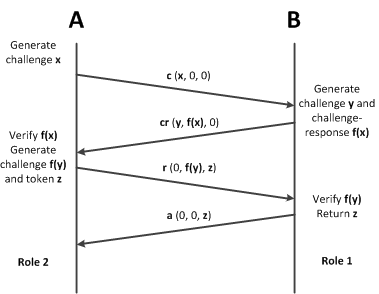
\includegraphics{images/4way_handshake.png}
	\caption{A complete 4-way handshake}
	\label{fig:4way_handshake}
\end{figure}

\noindent
\\\\
The first step in the 4-way handshake is to send an OGM with a challenge value which is adequately named Challenge message. This challenge value corresponds to the nonce value in message II in the authentication handshake, as proposed in Section \ref{authentication_handshake}.
\\\\
The node receiving the Challenge message will generate and send a Challenge-Response message with a new challenge value and the response value set as a function of the challenge received, which corresponds to message III in the authentication handshake. The function used here corresponds to the encrypted hash-function of the nonce.
\\\\
If the receiving node verifies the response, it returns a Response message where the response value set as a function on the received challenge in the Challenge-Response message. In addition the message is appended an authentication value to be used as the authentication token in the network. These messages loosely corresponds to message IV and VI in \ref{authentication_handshake}, except that the authentication value sent is going to be used as a signature later, whereas the proxy certificate sent in message VI is used to make individual signatures.
\\\\
The node that sent the Response message now waits for the other node to send an OGM with the same authentication value as a confirmation that he has received the token. If the correct message is received the 4-way handshake is complete and the authentication value, will be saved and used in every OGM from this point on and we refer to this only as OGM messages. The same node also sets his role to two, becoming the master node, given it was not the master from the very outset.
\\\\
The other node, upon reception of the Response message, also saves this authentication token value, and sets its role to one, becoming an authenticated node.

\subsection{Detailed Authentication Description}
The 4-way handshake is triggered whenever an unauthenticated node or the master node receives an OGM with the challenge, response, and authentication values set to zero. These messages we call Plain OGMs. 
\\\\
The challenge values are always set by generating a numbers with a pseudo-random number generator (PRNG). The function used to generate response values is very simple since it multiplies the challenge by two modulo of the largest possible number. For our actual system design these functions would be replaced with a stronger cryptographic algorithm based on public key cryptography.
\\\\
The master node will not accept any messages from nodes authenticated in other networks. That is, messages that contain an authentication value greater than zero, but different from the masters token will be discarded. The master node will also drop any Challenge-Response OGMs it may receive.
\\\\
For simplicity, we have chosen to let all authenticated nodes discard messages with a different or zero values in the authentication token. This means that new nodes have to be direct neighbor of the master node to be able to authenticate themselves.

\subsubsection*{Random Back-off}
Because we have not implemented a stand-alone authentication protocol using a separate socket, we added our handshake values to the OGMs being scheduled by the BATMAN protocol. We where reluctant to alter the message flow as this would change the mode of operation of the whole BATMAN OGM scheduling which might cause unintentional consequences for the routing.
\\\\
We quickly realized that when two unauthenticated nodes discover each other with Plain OGMs, a 4-way handshake will be triggered at both nodes approximately at the same time. For this reason we included a random back-off function which makes a node back off from sending Challenges when a handshake collision is detected. That is, if a node sends a challenge, but receives a challenge before the handshake is complete, the node will generate a random back-off time of less than 10 seconds.
\\\\
The back-off function does not halt other operations of BATMAN, it only clears all challenge and response values and make sure no new challenge is to be sent before the random back-off time expired. If the node receives a Challenge before his back-off time is expired, he replies to the as usual with a Challenge-Response.
\\\\
However, this back-off time does not completely solve the problem. After a node has detected a collision and sets its random back-off time, it will still continue to receive at least a few more identical Challenges because of the high frequency in which the OGMs are scheduled and sent at the other node. These Challenges should also be discarded thus we made a quick fix by not allowing any Challenges to be processed before half the random back-off time has passed. Figure \ref{fig:4way_handshake_backoff} illustrates this problem. The red field in the figure indicates the period in which no challenges are accepted after a collision.

\begin{figure}[ht]
	\centering
		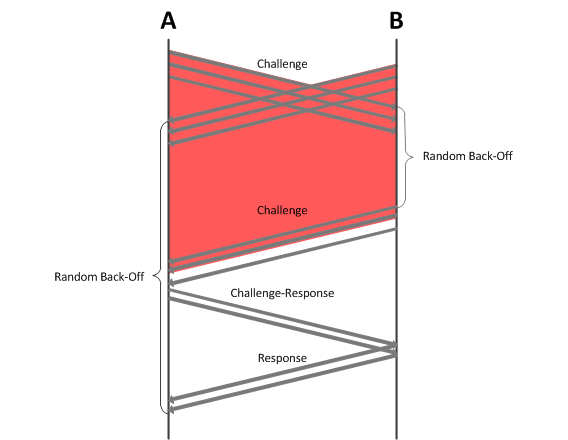
\includegraphics{images/4way_handshake_backoff.png}
	\caption{Back-off in the handshake algorithm. Node A only accepts Bs challenges halfway through the random back-off time}
	\label{fig:4way_handshake_backoff}
\end{figure}

\noindent
\\\\
This is however not a very efficient way of dealing with the problem and creates unnecessary delay in the authentication process. But if the functionality is moved into separate authentication protocol this could be avoided. We have decided to do this with the handshakes in our system design, see \ref{am_handshake}. We will however test our implementation and get some numbers which we can compare.


